\newcommand\minilogo{
  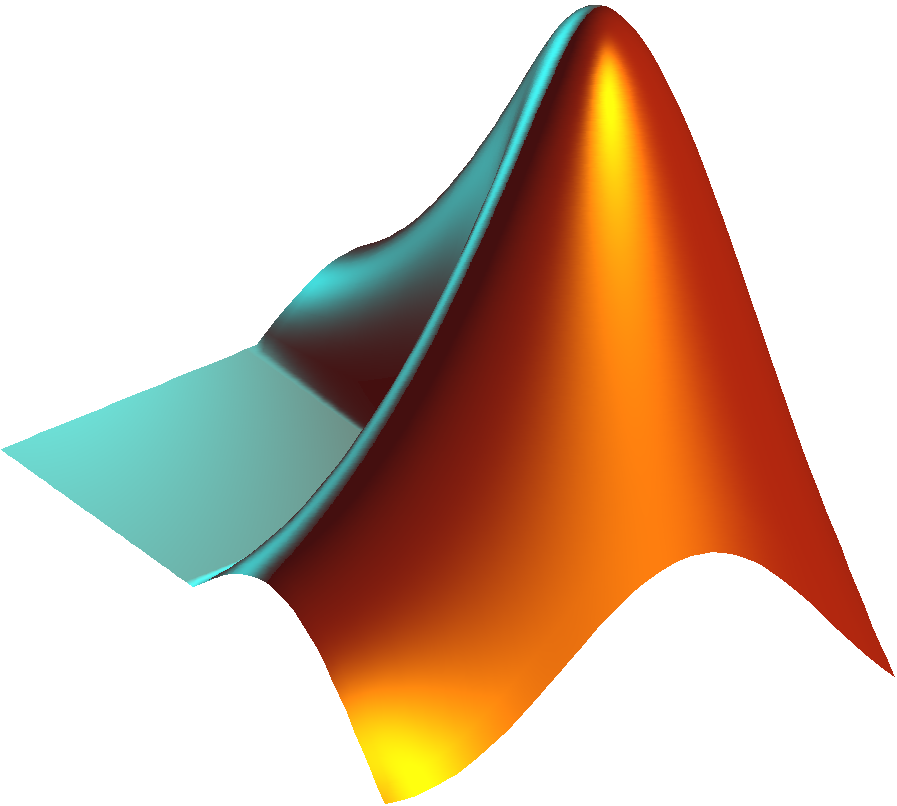
\includegraphics[width=0.5cm]{./media/Matlab_Logo.png}
}

\mode<article>
{
En lo que sigue daremos una revisión
de los elementos de programación 
mínimos necesarios para esta materia.
El lenguaje de programación oficial ha ido mutando con los años. Inicialmente se usó \texttt{FORTRAN } 
pues era el lenguaje más utilizado en programación científica. 
Desde el año 2012 utilizamos MATLAB por su curva de aprendizaje más amigable aunque su costo monetario fue siempre considerable.
Encontrará en este apunte muchos de los ejemplos que usábamos para este lenguaje. 

Desde el 2019 comenzamos a experimentar con \texttt{Python} por varias razones. 
En primer lugar se trata de una herramienta de código abierto y libre, i.e. gratis. 
Esto facilita la distribución entre los alumnos y el acceso a material de estudio. 
En segundo lugar, y quizá con mayor importancia, en los últimos diez años la adopción de este lenguaje de programación en la comunidad técnica y científica ha sido abrumadora. 
Todas las herramientas actuales tienen alguna interfaz a python o se desarrollan directamente en este lenguaje.
Nos vemos entonces en la obligación de mantenernos actualizados este aspecto. 

Sin embargo los métodos numéricos no son dependientes del lenguaje de programación elegido. 
Al mismo tiempo los conceptos de programación que repasaremos a continuación pueden generalizarse a cualquier lenguaje con diferencias en la sintaxis como veremos a continuación. 


%\texttt{MATLAB}
%\footnote{
%Esto puede estar en cambio. Recientemente hemos
%ampliado nuestro interes en Python debido a la
%amplia disponibilidad de entornos libres y de código 
%abierto, sino también por el alto grado de incorporación
%en el ambiente profesional durante los últimos tiempos.
%}
%, no solo por razones
%históricas, sino por su accesibilidad
%para profesionales sin experiencia previa
%en programación. En los casos donde sea posible, 
%se darán las indicaciones equivalentes 
%en otros lenguajes de uso corriente en la material 


% \begin{figure}
% \includeslide{FrameVentanaMatlab}
% \caption{Ventana de Matlab. se observan 
% el arbol de archivos del directorio
% de trabajo, el editor de guiones
% y la línea de comandos. 
% \label{FigMatlabInicio} }
% \end{figure}
}

\subsection{Entorno de desarrollo}

\mode*

\begin{frame}<presentation>[label=FrameMatlabPrimero]{Primeros Pasos en Matlab}
\begin{itemize}
\item[\minilogo] MATrix LABoratory
\item[\minilogo] Multiplataforma
\item[\minilogo] \url{http://www.mathworks.com/products/matlab}
\item[\minilogo] Lenguaje de programación, consola progrmable, ejecucion y redacción de scripts (guiones).
\end{itemize}
\end{frame}


\begin{frame}[label=FrameVentanaMatlab]
\frametitle<presentation>{Aspecto del Escritorio de Matlab}
%\mode<presentation>{
\begin{figure}
\begin{center}
\begin{tikzpicture}
\node [anchor=south west] (image) at (0,0) {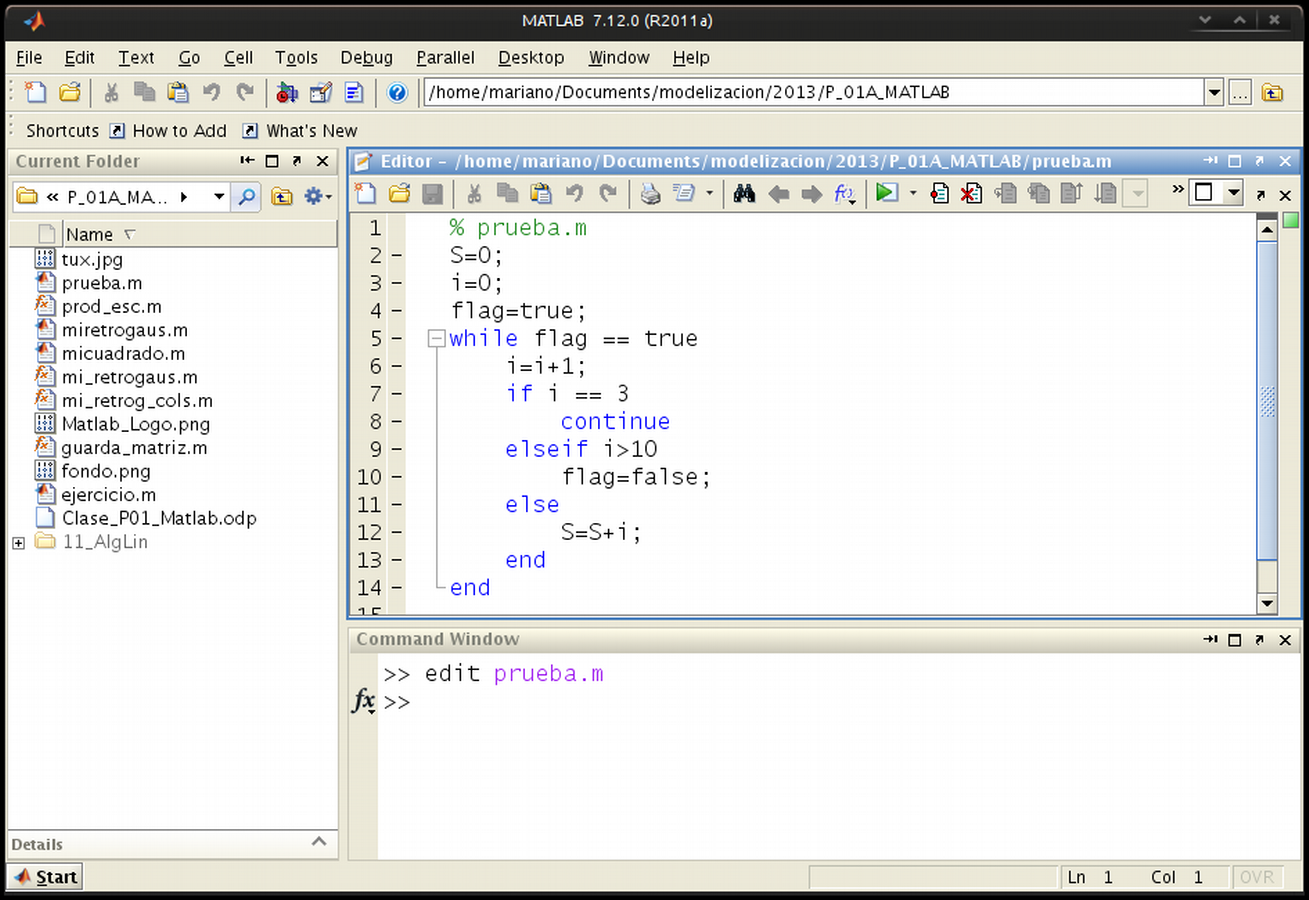
\includegraphics[width=0.7\textwidth]{./media/02-escritorio.png}};
\begin{scope}[x={(image.south east)},y={(image.north west)}]
  \node [rectangle,thick,fill=white,draw=black] at (0.15,0.2) {\small Archivos};
  \node [rectangle,thick,fill=white,draw=black] at (0.7,0.2) {\small  linea de comandos };
  \node [rectangle,thick,fill=white,draw=black] at (0.7,0.7) {\small  Editor de guiones };
\end{scope}
\end{tikzpicture}
\mode<article>{
 \caption{Ventana de Matlab. se observan 
 el árbol de archivos del directorio
 de trabajo, el editor de guiones
 y la línea de comandos. 
 \label{FigMatlabInicio}
  }
}
\end{center}
\end{figure}
%}
 
\end{frame}

\mode<article>
{
  El \texttt{entorno de desarrollo} (IDE) es la ``ventana''  en la cual se desarrolla la actividad de programación.
 Por ejemplo al iniciar MATLAB en cualquier plataforma, se observan las ventanas de la 
 \autoref{FigMatlabInicio}. Revise las configuraciones para obtener
el escritorio que le sea cómodo. Sin embargo, puede encontrar de 
 utilidad un escritorio como el que se muestra. 

 Si bien especificamos las indicaciones para esta herramienta 
 en particular, la estructura general vale para cualquier IDE que pueda encontrar.
 Busque por ejemplo el entorno \emph{PyCharm} para  \textbf{Python}, sus funcionalidades son   prácticamente idénticas.
}


\subsubsection{Notebooks}

En los últimos años se utiliza cada vez mas otro tipo de IDE a los que se denomina \texttt{Notebooks}.
Esta idea no es nueva, ya que este tipo de entornos se utilizaban ya en paquetes como el Mathemática.
Entre las ventajas de estos entornos puede encontrarse que permiten la escritura de texto con formato con sintaxis \texttt{Markdown} y \LaTeX \quad en un mismo documento donde se ejecutan piezas de código de varios lenguajes. 
Veremos el ejemplo de un \texttt{Jupyter Notebook} con kernel de \texttt{ Python } pero también \texttt{MATLAB} permite utilizar \texttt{Notebooks}. 
La particularidad de un \texttt{Jupyter Notebook} es que se ejecuta en un navegador web, y podemos ver su aspecto general en la \autoref{FigNotebook}

\mode*

\begin{frame}[label=FrameVentanaNotebook]
\frametitle<presentation>{Aspecto de un Notebook}
%\mode<presentation>{
\begin{figure}
\begin{center}
\begin{tikzpicture}
\node [anchor=south west] (image) at (0,0) {\includegraphics[width=0.7\textwidth]{./media/JupyerNotebook.png}};
\begin{scope}[x={(image.south east)},y={(image.north west)}]
  \node [rectangle,thick,fill=white,draw=black] at (0.1,0.2) {\small Archivos};
  \node [rectangle,thick,fill=white,draw=black] at (0.7,0.2) {\small  output de celda de código };
  \node [rectangle,thick,fill=white,draw=black] at (0.7,0.6) {\small  celda de código };
  \node [rectangle,thick,fill=white,draw=black] at (0.8 ,0.8) {\small  celda Markdown };
\end{scope}
\end{tikzpicture}
\mode<article>{
 \caption{Aspecto de un Notebook. Se observan 
  el árbol de archivos del directorio  de trabajo, las celdas de código y de texto (Markdown) y el output luego de la ejecución del código. 
 y la línea de comandos. 
 \label{FigNotebook}
  }
}
\end{center}
\end{figure}
%}
 
\end{frame}
\mode<all>
